% !TeX root = ../../main.tex
\subsection{平行線と角}

この単元で学習する角の種類は3種類である. それは \fitblankbf[対頂角]{}, \fitblankbf[同位角]{}, \fitblankbf[錯角]{} である.

\begin{definitionbox}{\textbf{対頂角}}
    \label{def:対頂角}
    2直線が交わるとき, その交点の周りには4つの角ができる. このうち
    \fitblankbf[向かい合っている]{} 2つの角を \fitblankbf[対頂角]{} という.
\end{definitionbox}

対頂角を図で表すと以下のようになる. また, そこから次のことが分かる.
\vspace{2em}
\begin{center}
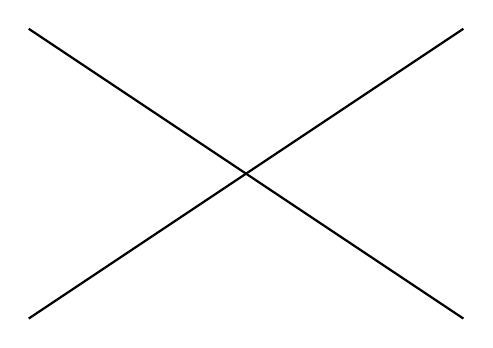
\begin{tikzpicture}[scale=1.15]
    \draw[thick] (-2.4,-1.6) -- (2.4,1.6);
    \draw[thick] (-2.4,1.6) -- (2.4,-1.6);
\end{tikzpicture}
\figcap{fig:対頂角}{対頂角}
\end{center}

\begin{theorembox}{\textbf{対頂角の性質}}
    \label{thm:対頂角}
    対頂角は \fitblankbf[いつでも]{} 等しい.
\end{theorembox}
\vspace{1em}

Theorem \ref{thm:対頂角} より, 図\ref{fig:対頂角} において \fitblankbf[\angle a = \angle c]{}, \fitblankbf[\angle b = \angle d]{} が成り立つ.

\newpage

\begin{definitionbox}{\textbf{同位角}}
    \label{def:同位角}
    2直線に1つの直線が交わるとき, その交点の同じ側にできる角を \fitblankbf[同位角]{} という.
\end{definitionbox}

\begin{definitionbox}{\textbf{錯角}}
    \label{def:錯角}
    2直線に1つの直線が交わるとき, その交点の反対側にできる角を \fitblankbf[錯角]{} という.
\end{definitionbox}

同位角と錯角を図で表すと以下のようになる. また, そこから次のことが分かる.
\vspace{2em}

\begin{center}
\begin{tikzpicture}[scale=0.9]
    \coordinate (LtopA) at (-3.2,1.1);
    \coordinate (LtopB) at (3.2,1.1);
    \coordinate (LbotA) at (-2.8,-0.9);
    \coordinate (LbotB) at (3.4,0.3);
    \coordinate (tA) at (-1.2,2.2);
    \coordinate (tB) at (2.4,-2.0);
    \draw[thick] (LtopA) -- (LtopB) node[right] {$\ell$};
    \draw[thick] (LbotA) -- (LbotB) node[right] {$m$};
    \draw[thick] (tA) -- (tB) node[below right] {$n$};
    \coordinate (P) at (intersection of LtopA--LtopB and tA--tB);
    \coordinate (Q) at (intersection of LbotA--LbotB and tA--tB);
    \fill (P) circle (1.2pt);
    \fill (Q) circle (1.2pt);
\end{tikzpicture}
\figcap{fig:同位角と錯角}{同位角と錯角}
\end{center}

\vspace{1em}
錯角は \fitblankbf[Z]{}, その鏡文字の \fitblankbf[S]{} の内側にできる角と考えると良い.

\begin{theorembox}{\textbf{同位角と錯角の性質①}}
    \label{thm:同位角と錯角の性質①}
    同位角と錯角は, いつでも等しい \fitblankbf[とは限らない]{} .
\end{theorembox}

\begin{theorembox}{\textbf{同位角と錯角の性質②}}
    \label{thm:同位角と錯角の性質②}
    2直線が \fitblankbf[平行]{} ならば同位角, 錯角はそれぞれ \fitblankbf[等しい]{}.

    また, これはその逆も成り立つ. すなわち,

    同位角, 錯角が等しい ならば 2直線は \fitblankbf[平行]{} である.
\end{theorembox}

Theorem \ref{thm:同位角と錯角の性質②} を図示すると以下のようになる.

\vspace{2em}
\begin{center}
\begin{tikzpicture}[scale=0.9]
    \coordinate (LtopA) at (-3.2,1.0);
    \coordinate (LtopB) at (3.2,1.0);
    \coordinate (LbotA) at (-3.2,-1.0);
    \coordinate (LbotB) at (3.2,-1.0);
    \coordinate (tA) at (-1.5,2.2);
    \coordinate (tB) at (1.5,-2.2);
    \draw[thick] (LtopA) -- (LtopB) node[right] {$\ell$};
    \draw[thick] (LbotA) -- (LbotB) node[right] {$m$};
    \draw[thick] (tA) -- (tB) node[below right] {$n$};
    % 平行マーク（$\ell$, $m$・各1つ）
    \draw[semithick] (-2.4,1.07) -- (-2.2,1.0) -- (-2.4,0.93);
    \draw[semithick] (-2.4,-0.93) -- (-2.2,-1.0) -- (-2.4,-1.07);
    \coordinate (P) at (intersection of LtopA--LtopB and tA--tB);
    \coordinate (Q) at (intersection of LbotA--LbotB and tA--tB);
    \fill (P) circle (1.2pt);
    \fill (Q) circle (1.2pt);
\end{tikzpicture}
\figcap{fig:同位角と錯角の性質}{同位角と錯角の性質}
\end{center}
\vspace{1em}

Theorem \ref{thm:同位角と錯角の性質②} より, 図\ref{fig:同位角と錯角の性質} において
\fitblankbf[\angle a = \angle c]{}, \fitblankbf[\angle b = \angle d]{} が成り立つ.

\newpage
